The application follows an object oriented approach. To unify the implementation of all cluster algorithms a base class, not meant for actual instanceing, was defined aggregateing all functions that the cluster algorithms need.
The cluster algorithms themselves are implemented as child classes inheriting all methods and attributes from the base clustering class. This allows setting different parameters for every cluster algorithm while guaranteeing the existence and uniform execution of methods used by all algorithms.

\begin{figure}[H]
    \centering
    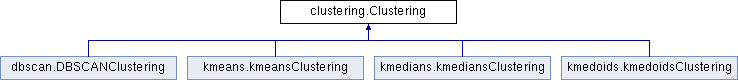
\includegraphics[width=0.9\textwidth]{../docs/html/classclustering_1_1Clustering}
    \caption{Inheritance diagramm for the cluster algorithm classes}
\end{figure}

Three different libraries were used for their implementations of the used cluster algorithms. 
For K-Means and K-Medians the pyclustering \cite{Novikov2019} implementations were used, because of their flexibility in setting custom distance measures. For K-Medoids the scikit learn extra \cite{scikit-learn-extra} implementation was used.
DBSCAN is realised using the scikit learn implementation \cite{scikitlearn}.

To reduce time spent on computing a class for organising already calculated resulsts as json files was created. All clustering results using the option of a predefined fixed seed are, if available, loaded from a file, or are calculated and then saved. Optionally cluster results can be bulk computed using a given script (\textit{result\_calculation.py}). Because of the large amount of possible parameter combinations of DBSCAN we decided to precompute only results for K-Means, K-Medians and K-Medoids with $k$ ranging from 1 to 10 for all distance measures.

The calculation of cluster indices is packaged into a Indices class and uses scikit learn implementations of the different scoring methods. Clustering results used for index calculations are saved using a data structure called SessionState. This structure is written by Thiago Teixeira \cite{sessionstate} implementing a way of saving parameters per session. That is for example a browser tab in which the interface is opened. The variables saved in the SessionState are persistent until a session is closed, eventhough streamlits framework is designed in a way, where every page is a sequential python script being completely reloaded when an action is triggered. 

Finally the webfrontend is implemented using streamlit and is hosted using their sharing service \footnote{\scriptsize\url{https://share.streamlit.io/elpelt/datascience1_group42/main/code/web_frontend.py}}. The cluster plots are generated using either seaborn or altair given a flag one can set in the frontend. The scoring results are visualised using matplotlib. The graphs which are visualised using altair are interactive in the way, that the user can freely move and zoom through the plots. By hovering over a point informations about this plot are shown in a small popup window. Where possible streamlits cacheing decorator is used, to reduce loading times when using any widget on the webpage.

Additionally the DBSCAN heuristic described in section \ref{dbscanheuristic} was also implemented using streamlit and interactive altair charts for displaying the results. All utility functions for the heruistic were packaged into a class and are then called from the script implementing the frontend. The finished page is also hosted on streamlit share \footnote{\scriptsize\url{https://share.streamlit.io/elpelt/datascience1_group42/main/code/heuristic_web.py}} and is linked to from the projects webfrontend, when choosing DBSCAN as clustering algorithm.

All of the code base for the project is documented using the Doxygen style and an automatically generated documentation containing detailed description of every class, method and attribute can be accessed through the github projects page \footnote{\scriptsize\url{https://elpelt.github.io/datascience1_group42}}.